%%%%%%%%%%%%%%%%%%%%%%%%%%%%%%% document and size %%%%%%%%%%%%%%%%%%%%%%%%%%%%%%
\documentclass[10pt]{beamer}

%%%%%%%%%%%%%%%%%%%%%%%%%%%%% special libraries %%%%%%%%%%%%%%%%%%%%%%%%%%%%%%%%
\usepackage{ngerman}
\usepackage{tikz}
\usetikzlibrary{arrows,automata}
\usepackage{fancyhdr}
\usepackage[export]{adjustbox}
\usepackage{lipsum}
\usepackage{lmodern}
\usepackage{tabularx}
\usepackage{array}
\usepackage{amsmath}
\usepackage{stmaryrd}
\usepackage{algorithmic}
\usepackage[]{algorithm2e}
\usepackage{colortbl}
%%%%%%%%%%%%%%%%%%%%%%%%%%%%%% custum commands %%%%%%%%%%%%%%%%%%%%%%%%%%%%%%%%%
\newcommand{\gap}{\ \\ \ \\}
\definecolor{GreenTOL}{HTML}{225522}
%%%%%%%%%%%%%%%%%%%%%%%%%%%%%%%%% DO NOT TOUCH %%%%%%%%%%%%%%%%%%%%%%%%%%%%%%%%%
% setup of the metropolis theme
\setbeamerfont{footnote}{size=\scriptsize}
\setbeamertemplate{footline}{}
\setbeamercolor{footnote}{fg=white,bg=mDarkTeal}

\usetheme[progressbar=frametitle]{metropolis}
\usepackage{appendixnumberbeamer}

\usepackage{booktabs}
\usepackage[scale=2]{ccicons}

\usepackage{pgfplots}
\usepgfplotslibrary{dateplot}

\usepackage{xspace}
\newcommand{\themename}{\textbf{\textsc{metropolis}}\xspace}

% thick lines
\tikzset{every picture/.style={line width=1.5pt}} 

% for the title page
\title{Der linearzeit MST-Algorithmus}
\subtitle{Der schnellste Algorithmus f"ur das MST/ MSF Problem}
\date{}
\author{Max Springenberg}
\institute{Proseminar: Randomisierte Algorithmen, TU Dortmund}
%%%%%%%%%%%%%%%%%%%%%%%%%%%%%%%%%%%%%%%%%%%%%%%%%%%%%%%%%%%%%%%%%%%%%%%%%%%%%%%%

\begin{document}

\maketitle

%% Ablauf:
% 1. Intro:
%   Motivation
%!TEX root = ../compehension.tex
\section{Motivation}

\subsection{Konventionen}
In dieser Ausarbeitung wird sich an die "ublichen Konventionen zur Notation
    von Variablen in Graphen orientiert. So definieren wir einen Graphen als
    $G = (V,E)$, mit der Anzahl von Knoten $n = |V|$ und Kanten $m = |E|$.
    Ferner betrachten wir ungerichtete gewichtete Graphen und bezeichnen 
    die Gewichtungsfunktion als $w: E \rightarrow \mathbb{R}$.\\

\subsection{MST und MSF}
Der minimale Spannbaum, oder auch MST, stellt einen azyklischen 
    zusammenh"angenden Teilgraph aus G, der alle Knoten verbindet und
    dessen Summe von Kantengewichte $\sum_{e \in E_{MST}} w(e)$
    minimal ist dar.\\
Ist G selbst nicht zusammenh"angend, so werden wir einen minimalen Spannwald
    als n"achst beste L"osung betrachten.
    Ein minimaler Spannwald besteht aus einer Sammlung von minimalen 
    Spannb"aumen f"ur die verbundenen Komponenten in G.\\

\subsection{Warum ein nichtdeterministischer Anzatz von Vorteilen sein kann}

Wir werden in dieser Ausarbeitung zum Kapitel 10.3 aus dem Buch
    `Randomized Algorithms` von Motwani, R., Raghavan, P.  
    einen
    randomisierten Ansatz f"ur einen Algorithmus, der einen minimalen Spannbaum
    in erwarteter Linearzeit aproximiert betrachten.\\
Das MST Problem ist in $P$, und es sind bereits 
    deterministische Algorithmen wie die von
    Prim, Kruskal, Bor\r uvka bekannt
    , die mit einer Worst-Case Laufzeitschranke 
    von $O(m * log(n))$ das Problem l"osen.
    Zudem existiert der Algorithmus von Bernard Chazelle, f"ur den eine
    Worst-Case Laufzeitschranke von $O(m * log \beta(m,n))$ bekannt ist, wobei
    mit
    $\beta(m,n) = \{i | log^{(i)} n \leq m / n\}$ die inverse Ackermann Funktion
    verwendet wird. 
    $log^{(i)} n$ ist hierbei die $i$-te Anwendung von $log$ auf $n$.
    Dementsprechend steigt die Funktion $\beta$ so schwach, dass die
    aus ihr resultierenden Faktoren f"ur die Worst-Case Laufzeit hinsichtlich
    der Gr"o"se von Graphen in der Praxis als nahezu konstant angesehen werden.\\
Wozu dient also ein nichtdeterministischer Algorithmus, der im Erwartungswert 
    linear verl"auft?
    - Die Antwort auf diese Frage kann sowohl durch die komplexe Implementierung
    des Algorithmus von Chazelle, als auch der Stabilit"at, bzw. G"ute,
    des vorgestellten Algorithmus hinsichtlich seiner Laufzeit
    und nicht zuletzt durch das Betrachten des Algorithmus als akademisches
    Beispiel f"ur kreative Laufzeitverbesserungen begr"undet werden.\\

%   MST und Kontext/ vllt. Konventionen
% 1. Intro:
% vllt. Konventionen an die Tafel
\section{Was wollen wir erreichen?}
% MST
\begin{frame}{MST}
    \begin{overlayarea}{\textwidth}{4cm}
        \begin{center}
        \begin{tikzpicture}
            \node[state](A) at (0,0)  {A};
            \node[state](B) at (3,0)  {B};
            \node[state](C) at (0,-3) {C};
            \node[state](D) at (3,-3) {D};
            \node[state](E) at (6,0)  {E};
            \node[state](F) at (9,0)  {F};
            \node[state](G) at (9,-3) {G};
            \node[state](H) at (6,-3) {H};
            \only<1>{\path
                (A) 
                    edge [-, above] node {6}  (B)
                    edge [-, left ] node {7}  (C)
                (B)                                        
                    edge [-, left ] node               {8}  (C)
                    edge [-, left ] node {11} (D)
                (D)                                        
                    edge [-, left ] node {12} (E)
                    edge [-, below] node               {13} (H)
                (E)                                        
                    edge [-, above] node {6}  (F)
                    edge [-, left ] node               {8}  (G)
                    edge [-, left ] node               {10} (H)
                (F)                                        
                    edge [-, left ] node {7}  (G)
                (G)                                        
                    edge [-, below] node {7}  (H)
                ;}
            \only<2>{\path
                (A) 
                    edge [-, above, color=orange] node {6}  (B)
                    edge [-, left , color=orange] node {7}  (C)
                (B)                                        
                    edge [-, left ] node               {8}  (C)
                    edge [-, left , color=orange] node {11} (D)
                (D)                                        
                    edge [-, left , color=orange] node {12} (E)
                    edge [-, below] node               {13} (H)
                (E)                                        
                    edge [-, above, color=orange] node {6}  (F)
                    edge [-, left ] node               {8}  (G)
                    edge [-, left ] node               {10} (H)
                (F)                                        
                    edge [-, left , color=orange] node {7}  (G)
                (G)                                        
                    edge [-, below, color=orange] node {7}  (H)
                ;}
        \end{tikzpicture}
        \end{center}
    \end{overlayarea}
\end{frame}

\begin{frame}{MSF}
    \begin{overlayarea}{\textwidth}{4cm}
        \begin{center}
        \begin{tikzpicture}
            \node[state](A) at (0,0)  {A};
            \node[state](B) at (3,0)  {B};
            \node[state](C) at (0,-3) {C};
            \node[state](D) at (3,-3) {D};
            \node[state](E) at (6,0)  {E};
            \node[state](H) at (6,-3) {H};
            \node[state](F) at (9,0)  {F};
            \node[state](G) at (9,-3) {G};
            \only<1>{
            \path
                (A) edge [-, above] node {6} (B)
                    edge [-, left ] node {7} (C)
                (B)
                    edge [-, left] node {8} (C)
                (D)
                    edge [-, left ] node {12} (E)
                    edge [-, below] node {13} (H)
                (E)
                    edge [-, left ] node {10} (H)
                ;
            }
            \only<2>{
            \path
                (A) edge [-, above, color=orange] node {6} (B)
                    edge [-, left , color=orange] node {7} (C)
                (B)
                    edge [-, left] node {8} (C)
                (D)
                    edge [-, left , color=orange] node {12} (E)
                    edge [-, below] node {13} (H)
                (E)
                    edge [-, left , color=orange] node {10} (H)
                ;
            }
        \end{tikzpicture}
        \end{center}
    \end{overlayarea}
\end{frame}



%
% 2. F-leicht/ -schwer:
\section{$F$-schwere/-leichte Kanten}

$F$-schwere und -leichte Kanten sind ein wesentlicher Bestandteil des 
    MST-Algorithmus. Mittels der Identifizierung von Kanten in einem Graphen $G$
    als $F$-schwer hinsichtlich eines Waldes $F$ in $G$ kann
    bereits entschieden werden, dass diese Kante nicht im MST von $G$ enthalten
    ist. Der Umkehrschluss f"ur $F$-leichte Kanten gilt jedoch nicht, wie wir
    sehen werden.
    Betrachten wir also eine Approximation $F$ eines MST bez"uglich $G$, so k"onnen
    wir neben dem Gewicht des Waldes auch die Anzahl $F$-leichten Kanten als
    G"utema"s verwenden.\\

\subsection{Definition}

Wir betrachten neben der Gewichtungsfunktion $w$ nun die Funktion $w_F$, mit
    $$
    w_F(\{u,v\}) =  \begin{cases}
                        \infty, P(\{u,v\}) = \emptyset\\
                        max\{w(P_e(\{u,v\}))\}, \text{ sonst}
                    \end{cases}
    $$
, wobei $w(P_e(\{u,v\}))$ bedeutet, dass $w$ auf alle Kanten des Pfades angewandt
    wurde.\\
$w_F$, gibt also das Kantengewicht der Kante mit maximalen Gewicht auf dem
    Pfad von $u$ nach $v$ in $F$ aus. Sollte dieser Pfad nicht existieren, so
    nehmen wir an, dass diese Kante unendlich schwer ist.\\
Ist das Gewicht einer Kante $w(e)$ echt gr"o"ser als das maximale Gewicht auf dem 
    Pfad $P_e(e)$ in $F$, bzw. $w(e) > w_F(e)$, 
    so bezeichnen wir sie als $F$-schwer.
    Sonst ist sie $F$-leicht.

\subsection{Informationsgewinn durch $F$-schwere Kanten}

Wir haben bereits erw"ahnt, dass $F$-schwere Kanten nicht in einem MSF, bzw. MST
    enthalten sein k"onnen.
    Dies werden wir im folgenden Beweisen.
    Aufbauend darauf k"onnen wir dann einen Verifikationsalgorithmus definieren.\\

\subsubsection{Beweis}
\label{sec:fProof}

Sei $F$ ein beliebiger Baum in $G$.
    Existiert eine $F$ schwere Kante in $G$, $e=\{u, v\}$, so gelten folgende 
    Eigenschaften f"ur $F$:\\
(i) Es existiert ein Pfad zwischen $u$ und $v$\\
(ii) Die Gewichtung jeder Kante auf dem Pfad ist leichter als $w(e)$\\
W"are $e$ im $MSF$ von $G$ enthalten, so w"urde das Tauschen einer Kante aus
    $F$ durch $e$ die Approximation $F$ verbessern.\\
Aus (i) folgt, dass durch $e$ ein Zyklus entsteht. Insbesondere bedeutet das, 
    dass wir f"ur $e$ eine Kante auf dem Pfad zwischen $u$ und $v$ tauschen
    m"ussten.
    Aus (ii) folgt jedoch, dass dies $F$ verschlechtern w"urde.
    Damit kann $e$ nicht im MSF von $G$ enthalten sein.\\
Der Umkehrschluss, dass alle $F$-leichten Kanten im MSF vorkommen gilt jedoch
    nicht.
    Betrachten wir beispielsweise einen vollst"andigen Graphen $G_{w_1}$ mit der 
    Gewichtungsfunktion $w(e) = 1, \forall e \in E_{G_{w_1}}$ und 
    $n = |V_{G_{w_1}}| > 2$, so stellen wir fest, dass jeder Pfad in $G$, der alle
    Knoten verbindet ein MST $F$ von $G$ ist.
    Zudem ist jede Kante $F$-leicht, da alle Kanten gleich gewichtet werden.
    W"are jede $F$-leichte Kante im MST enthalten, so w"are der MST gleich $G$,
    da $G$ vollst"andig und $n > 2$ ist, w"are aber mindestens ein Zyklus im 
    MST enthalten und damit eine Baum-Eigenschaft verletzt.\\
    Damit gilt der Umkehrschluss nicht.\\
\\
Wir k"onnen also s"amtliche $F$-schwere Kanten f"ur das erfassen des MST 
    ignorieren, bzw. sogar aus $G$ eliminieren.\\
Diese Erkenntnis nimmt sich auch der MST-Algorithmus zum Nuzten. In gewisser
    Hinsicht werden wir den umgekehrten Ansatz von Kruskal, welcher Kanten nach
    gewichten aufsteigend sortiert und immer nur $F$-leichte Kanten hinzunimmt,
    durch das erfassen von $F$-schweren Kanten "uber Stichproben von W"aldern
    in $G$ verfolgen.\\

\subsubsection{Verifikation durch $F$-schwere/-leichte Kanten}
\label{sec:verification}
Es liegt nahe, dass $F$ kein MSF in $G$ ist, wenn eine Kante $\{u,v\}$ 
    existiert dessen gewicht echt kleiner als das des maximalen Gewichts auf dem
    Pfad $P_e(\{u,v\})$ in $F$ ist. W"urde man annehmen, dass $F$ ein MSF w"are, 
    so k"onnte man $E_F$ um die Kante $\{u,v\}$ erweitern und den dadurch 
    entstandenen Zyklus mittels entfernen der Kante maximalen Gewichts auf dem
    Pfad $P_e(\{u,v\})$ l"osen. Dadurch h"atte man die Zusammenh"angende 
    Komponente als solche gewahrt und eine schwerere durch eine leichtere Kante
    substituiert. Folglich h"atte man einen leichteren Wald und $F$ w"are damit
    kein MSF.\\
Diese Erkenntnis reicht bereits aus um einen Verifikationsalgorithmus zum 
    MST und MSF Problem zu konstruieren.
    So k"onnte man auf $F$ eine Tiefensuche durchf"uhren und f"ur jeden Pfad 
    das maximale Kantengewicht unter dem Start und Endknoten dessen mittels
    Hashing in einer Hashmap $w_F : E_F \rightarrow \mathbb{R}$ abspeichern die 
    $\infty$ ausgibt, wenn f"ur eine Kante kein Wert gesetzt wurde.
    Anschlie"send w"urde man "uber $E_G$ iterieren und sicherstellen, dass gilt
    $\forall e \in E_G: w(e) \leq w_F(e)$.\\
Man den Verfizierungsalgorithmus auch so anpassen, dass die F-schweren Kanten
    ausgegeben werden.
    Ferner l"auft der Algorithmus in linearzeit.\\

%   Beweis zu F-schweren und leichten Kanten
% erklaeren von F-leicht/-chwer
\begin{frame}{Teaser: $F$-schwer}
    \begin{overlayarea}{\textwidth}{4cm}
        \only<1>{Sei $G$:}
        \only<2>{Sei $F$:}
        \only<3>{Dann ist etwas an \textcolor{blue}{diesen Kanten} besonders.}
        \ \\
        \gap
        \begin{tikzpicture}
            \node[state](A) at (0,0)  {A};
            \node[state](B) at (3,0)  {B};
            \node[state](C) at (0,-3) {C};
            \node[state](D) at (3,-3) {D};
            \node[state](E) at (6,0)  {E};
            \node[state](F) at (9,0)  {F};
            \node[state](G) at (9,-3) {G};
            \node[state](H) at (6,-3) {H};
            \only<1>{\path
                (A) 
                    edge [-, above] node {6}  (B)
                    edge [-, left ] node {7}  (C)
                (B)                                        
                    edge [-, left ] node               {8}  (C)
                    edge [-, left ] node {11} (D)
                (D)                                        
                    edge [-, left ] node {12} (E)
                    edge [-, below] node               {13} (H)
                (E)                                        
                    edge [-, above] node {6}  (F)
                    edge [-, left ] node               {8}  (G)
                    edge [-, left ] node               {10} (H)
                (F)                                        
                    edge [-, left ] node {7}  (G)
                (G)                                        
                    edge [-, below] node {7}  (H)
                ;}
            \only<2>{\path
                (A) 
                    edge [-, above, color=orange] node {6} (B)
                    edge [-, left , color=orange] node {7} (C)
                (D)
                    edge [-, left , color=orange] node {12} (E)
                (E)
                    edge [-, left , color=orange] node {10} (H)
                ;}
            \only<3>{\path
                (A) 
                    edge [-, above, color=orange] node {6} (B)
                    edge [-, left , color=orange] node {7} (C)
                (B)                                        
                    edge [-, left, color=blue] node               {8}  (C)
                    edge [-, left ] node {11} (D)
                (D)                                        
                    edge [-, left , color=orange] node {12} (E)
                    edge [-, below, color=blue] node               {13} (H)
                (E)                                        
                    edge [-, above] node {6}  (F)
                    edge [-, left ] node               {8}  (G)
                    edge [-, left , color=orange] node {10} (H)
                (F)                                        
                    edge [-, left ] node {7}  (G)
                (G)                                        
                    edge [-, below] node {7}  (H)
                ;}
        \end{tikzpicture}
    \end{overlayarea}
\end{frame}

\begin{frame}{$F$-leicht/-schwer}
    Sei $e=\{u,v\}$, $P_e$ in $F$, $w$ von $G$\\
    \ \\
    $w_F(e) = \begin{cases}
        \infty& , u$ und $v$ in verschiedenen Komponenten$\\
                        \textcolor{orange}{max\{w(P_e(e))\}}&,$ sonst$
                     \end{cases}$\\
    \gap
    \gap
    \begin{tabular}{ll}
        F-schwer:   & $\textcolor{orange}{w(e) > w_F(e)}$\\
        \\
        F-leicht:   & $\textcolor{orange}{w(e) \leq w_F(e)}$\\
    \end{tabular}
\end{frame}

\begin{frame}{$F$-schwere Kanten im MSF?}
    \begin{overlayarea}{\textwidth}{4cm}
        \only<2>{Zyklus D$,$E$,$H$,$D$ \lightning$}
        \only<3>{$w(\{$D$,$H$\}) > w(\{$E$,$H$\})$}
        \only<4>{$w(\{$D$,$H$\}) > w(\{$D$,$E$\})$}\ \\
        \gap
        \begin{tikzpicture}
            \node[state](A) at (0,0)  {A};
            \node[state](B) at (3,0)  {B};
            \node[state](C) at (0,-3) {C};
            \node[state](D) at (3,-3) {D};
            \node[state](E) at (6,0)  {E};
            \node[state](F) at (9,0)  {F};
            \node[state](G) at (9,-3) {G};
            \node[state](H) at (6,-3) {H};
            \only<1>{\path
                (A) 
                    edge [-, above, color=orange] node {6} (B)
                    edge [-, left , color=orange] node {7} (C)
                (B)                                        
                    edge [-, left, color=blue] node               {8}  (C)
                    edge [-, left ] node {11} (D)
                (D)                                        
                    edge [-, left , color=orange] node {12} (E)
                    edge [-, below, color=blue] node               {13} (H)
                (E)                                        
                    edge [-, above] node {6}  (F)
                    edge [-, left ] node               {8}  (G)
                    edge [-, left , color=orange] node {10} (H)
                (F)                                        
                    edge [-, left ] node {7}  (G)
                (G)                                        
                    edge [-, below] node {7}  (H)
                ;}
            \only<2>{\path
                (A) 
                    edge [-, above, color=orange] node {6} (B)
                    edge [-, left , color=orange] node {7} (C)
                (B)                                        
                    edge [-, left ] node               {8}  (C)
                    edge [-, left ] node {11} (D)
                (D)                                        
                    edge [-, left , color=orange] node {12} (E)
                    edge [-, below, color=orange] node               {13} (H)
                (E)                                        
                    edge [-, above] node {6}  (F)
                    edge [-, left ] node               {8}  (G)
                    edge [-, left , color=orange] node {10} (H)
                (F)                                        
                    edge [-, left ] node {7}  (G)
                (G)                                        
                    edge [-, below] node {7}  (H)
                ;}
            \only<3>{\path
                (A) 
                    edge [-, above, color=orange] node {6} (B)
                    edge [-, left , color=orange] node {7} (C)
                (B)                                        
                    edge [-, left ] node               {8}  (C)
                    edge [-, left ] node {11} (D)
                (D)                                        
                    edge [-, left , color=orange] node {12} (E)
                    edge [-, below, color=blue] node               {13} (H)
                (E)                                        
                    edge [-, above] node {6}  (F)
                    edge [-, left ] node               {8}  (G)
                    edge [-, left , color=blue] node {10} (H)
                (F)                                        
                    edge [-, left ] node {7}  (G)
                (G)                                        
                    edge [-, below] node {7}  (H)
                ;}
            \only<4>{\path
                (A) 
                    edge [-, above, color=orange] node {6} (B)
                    edge [-, left , color=orange] node {7} (C)
                (B)                                        
                    edge [-, left ] node               {8}  (C)
                    edge [-, left ] node {11} (D)
                (D)                                        
                    edge [-, left , color=blue] node {12} (E)
                    edge [-, below, color=blue] node               {13} (H)
                (E)                                        
                    edge [-, above] node {6}  (F)
                    edge [-, left ] node               {8}  (G)
                    edge [-, left , color=orange] node {10} (H)
                (F)                                        
                    edge [-, left ] node {7}  (G)
                (G)                                        
                    edge [-, below] node {7}  (H)
                ;}
        \end{tikzpicture}
    \end{overlayarea}
\end{frame}

\begin{frame}{$F$-leichte Kanten im MSF?}
    $G_{w_1}$\only<2,3,4>{, MST \textcolor{orange}{$F$}}:\\
    \gap
    \begin{overlayarea}{\textwidth}{4cm}
        \begin{center}
            \begin{tikzpicture}
                \node[state](A) at (3,0)  {A};
                \node[state](B) at (6,-3)  {B};
                \node[state](C) at (0,-3) {C};
                \only<1>{\path
                    (A) 
                        edge [-, above] node {1} (B)
                        edge [-, left ] node {1} (C)
                    (B)                       
                        edge [-, above] node {1} (C)
                    ;}
                \only<2>{\path
                    (A) 
                        edge [-, above, color=orange] node {1} (B)
                        edge [-, left , color=orange] node {1} (C)
                    (B)                                        
                        edge [-, above] node {1} (C)
                    ;}
                \only<3>{\path
                    (A) 
                        edge [-, above, color=orange] node {1} (B)
                        edge [-, left ] node {1} (C)
                    (B)
                        edge [-, above, color=orange] node {1} (C)
                    ;}
                \only<4>{\path
                    (A) 
                        edge [-, above] node {1} (B)
                        edge [-, left , color=orange] node {1} (C)
                    (B)
                        edge [-, above, color=orange] node {1} (C)
                    ;}
            \end{tikzpicture}\\
        \end{center}
    \end{overlayarea}
\end{frame}

%   lineare Klassifikation erwaehnen, aber keinen Algorithmus vorstellen
%
% 3. Reduzieren des Graphen:
%   Einstieg: Teaser Rekursion
%   3.1 Boruvka:
%       Prinzip erklaeren
\section{Bor\r uvka Phasen}
\begin{frame}{Ablauf}
    \begin{enumerate}
        \item Kontraktierende Kanten markieren
        \item Verbundene Komponenten bestimmen
        \item Verbundene Komponenten durch einzelne Knoten ersetzen
        \item Selbstschleifen entfernen
    \end{enumerate}
\end{frame}
\begin{frame}{Ablauf}
    \begin{overlayarea}{\textwidth}{15cm}
        \gap
        \only<1>{1. Kontraktierende Kanten markieren}
        \only<2>{2. Verbundene Komponenten bestimmen}
        \only<3>{3. Verbundene Komponenten durch einzelne Knoten ersetzen}
        \only<4>{4. Selbstschleifen entfernen}
        \only<4>{\ \\ \gap}
        \begin{center}
        \begin{tikzpicture}[minND/.style={circle,
                                          anchor=center,
                                          draw=black,
                                          text width=2.5mm,
                                          inner sep=3pt,
                                          align=center}]
            \only<1>{
                \node[minND](A1) at (0,0) {$A_1$};
                \node[minND](A2) at (1,0) {$A_2$};
                                                 
                \node[minND](B1) at (3,0) {$B_1$};
                \node[minND](B2) at (4,0) {$B_2$};

                \node[minND](C1) at (0,-3) {$C_1$};
                \node[minND](C2) at (0,-4) {$C_2$};

                \node[minND](D1) at (3,-3) {$D_1$};
                \node[minND](D2) at (3,-4) {$D_2$};

                \node[minND](E1) at (6,0) {$E_1$};
                \node[minND](E2) at (7,0) {$E_2$};

                \node[minND](F1) at (9,0)  {$F_1$};
                \node[minND](F2) at (10,0) {$F_2$};

                \node[minND](G1) at (9,-3) {$G_1$};
                \node[minND](G2) at (9,-4) {$G_2$};

                \node[minND](H1) at (6,-3) {$H_1$};
                \node[minND](H2) at (6,-4) {$H_2$};
            }
            \only<2>{
                \node[minND, color=blue](A1) at (0,0) {$A_1$};
                \node[minND, color=blue](A2) at (1,0) {$A_2$};
                           , color=blue                      
                \node[minND, color=blue](B1) at (3,0) {$B_1$};
                \node[minND, color=blue](B2) at (4,0) {$B_2$};

                \node[minND, color=blue](C1) at (0,-3) {$C_1$};
                \node[minND, color=blue](C2) at (0,-4) {$C_2$};

                \node[minND, color=blue](D1) at (3,-3) {$D_1$};
                \node[minND, color=blue](D2) at (3,-4) {$D_2$};

                \node[minND, color=blue](E1) at (6,0) {$E_1$};
                \node[minND, color=blue](E2) at (7,0) {$E_2$};

                \node[minND, color=blue](F1) at (9,0)  {$F_1$};
                \node[minND, color=blue](F2) at (10,0) {$F_2$};

                \node[minND, color=blue](G1) at (9,-3) {$G_1$};
                \node[minND, color=blue](G2) at (9,-4) {$G_2$};

                \node[minND, color=blue](H1) at (6,-3) {$H_1$};
                \node[minND, color=blue](H2) at (6,-4) {$H_2$};
            }
            \only<3,4>{
                \node[state](A) at (0,0)  {A};
                \node[state](B) at (3,0)  {B};
                \node[state](C) at (0,-3) {C};
                \node[state](D) at (3,-3) {D};
                \node[state](E) at (6,0)  {E};
                \node[state](F) at (9,0)  {F};
                \node[state](G) at (9,-3) {G};
                \node[state](H) at (6,-3) {H};
            }

            \only<1>{\path
                (A1)
                    edge [-, above, color=blue] node {3} (A2)
                    edge [-, left ] node {7} (C1)
                (A2)
                    edge [-, above] node {6} (B1)
                (B1)
                    edge [-, above, color=blue] node {5} (B2)
                    edge [-, left ] node {8}  (C1)
                    edge [-, left ] node {11} (D1)
                (C1)
                    edge [-, left , color=blue] node {6} (C2)
                (D1)
                    edge [-, left , color=blue] node {10} (D2)
                    edge [-, left ] node {12} (E1)
                (D2)
                    edge [-, below] node {13} (H2)
                (E1)
                    edge [-, above, color=blue] node {1} (E2)
                    edge [-, left ] node {8} (G1)
                    edge [-, left ] node {10} (H1)
                (E2)
                    edge [-, above] node {6} (F1)
                (F1)
                    edge [-, above, color=blue] node {3} (F2)
                (F2)
                    edge [-, left ] node {7} (G1)
                (G1)
                    edge [-, left , color=blue] node {5} (G2)
                (G2)
                    edge [-, below] node {7} (H2)
                (H1)
                    edge [-, left , color=blue] node {4} (H2)
                ;}
                \only<2>{\path
                (A1)
                    edge [-, above, color=blue] node {3} (A2)
                    edge [-, left ] node {7} (C1)
                (A2)
                    edge [-, above] node {6} (B1)
                (B1)
                    edge [-, above, color=blue] node {5} (B2)
                    edge [-, left ] node {8}  (C1)
                    edge [-, left ] node {11} (D1)
                (C1)
                    edge [-, left , color=blue] node {6} (C2)
                (D1)
                    edge [-, left , color=blue] node {10} (D2)
                    edge [-, left ] node {12} (E1)
                (D2)
                    edge [-, below] node {13} (H2)
                (E1)
                    edge [-, above, color=blue] node {1} (E2)
                    edge [-, left ] node {8} (G1)
                    edge [-, left ] node {10} (H1)
                (E2)
                    edge [-, above] node {6} (F1)
                (F1)
                    edge [-, above, color=blue] node {3} (F2)
                (F2)
                    edge [-, left ] node {7} (G1)
                (G1)
                    edge [-, left , color=blue] node {5} (G2)
                (G2)
                    edge [-, below] node {7} (H2)
                (H1)
                    edge [-, left , color=blue] node {4} (H2)
                ;}
                \only<3>{\path
                (A) edge [-, above] node {6} (B)
                    edge [-, left ] node {7} (C)
                    edge [-, loop above, color=blue] node {3} (A)
                (B)
                    edge [-, left ] node {8} (C)
                    edge [-, left ] node {11} (D)
                    edge [-, loop above, color=blue] node {5} (B)
                (C)
                    edge [-, loop below, color=blue] node {6} (C)
                (D)
                    edge [-, left ] node {12} (E)
                    edge [-, below] node {13} (H)
                    edge [-, loop below, color=blue] node {10} (D)
                (E)
                    edge [-, above] node {6} (F)
                    edge [-, left ] node {8} (G)
                    edge [-, left ] node {10} (H)
                    edge [-, loop above, color=blue] node {1} (E)
                (F)
                    edge [-, left ] node {7} (G)
                    edge [-, loop above, color=blue] node {3} (F)
                (G)
                    edge [-, below] node {7} (H)
                    edge [-, loop below, color=blue] node {5} (G)
                (H)
                    edge [-, loop below, color=blue] node {4} (H)
                ;}
                \only<4>{\path
                (A) edge [-, above] node {6} (B)
                    edge [-, left ] node {7} (C)
                (B)
                    edge [-, left ] node {8} (C)
                    edge [-, left ] node {11} (D)
                (D)
                    edge [-, left ] node {12} (E)
                    edge [-, below] node {13} (H)
                (E)
                    edge [-, above] node {6} (F)
                    edge [-, left ] node {8} (G)
                    edge [-, left ] node {10} (H)
                (F)
                    edge [-, left ] node {7} (G)
                (G)
                    edge [-, below] node {7} (H)
                ;}
        \end{tikzpicture}
        \end{center}
    \end{overlayarea}
\end{frame}

%       Reduktion auf n/2 beweisen
\begin{frame}{Reduktion der Knoten}
    
\end{frame}

%   3.2 Stichproben:
%!TEX root = ./graph_reduction.tex
\subsection{Randomisierte Stichproben}

%       G(p) definieren, bzw. erklaeren
%       Reduktion auf m/2 erlaeutern
\begin{frame}{Kanten \glqq w"urfeln\grqq}
    \begin{overlayarea}{\textwidth}{4cm}
        \only<1>{$G_1:$}
        \only<2>{$G_1(p=0,5):$}
        \ \\ 
        \gap
        \begin{tikzpicture}
            \node[state](A) at (0,0)  {A};
            \node[state](B) at (3,0)  {B};
            \node[state](C) at (0,-3) {C};
            \node[state](D) at (3,-3) {D};
            \node[state](E) at (6,0)  {E};
            \node[state](H) at (6,-3) {H};
            \node[state](F) at (9,0)  {F};
            \node[state](G) at (9,-3) {G};
            \only<1>{\path
                    (A) 
                        edge [-, above] node {6}  (B)
                        edge [-, left ] node {7}  (C)
                    (B)                                        
                        edge [-, left ] node               {8}  (C)
                        edge [-, left ] node {11} (D)
                    (D)                                        
                        edge [-, left ] node {12} (E)
                        edge [-, below] node               {13} (H)
                    (E)                                        
                        edge [-, above] node {6}  (F)
                        edge [-, left ] node               {8}  (G)
                        edge [-, left ] node               {10} (H)
                    (F)                                        
                        edge [-, left ] node {7}  (G)
                    (G)                                        
                        edge [-, below] node {7}  (H)
 
                    ;}
            \only<2>{\path
                    (A) edge [-, above] node {6} (B)
                        edge [-, left ] node {7} (C)
                    (B)
                        edge [-, left ] node {8} (C)
                    (D)
                        edge [-, left ] node {12} (E)
                        edge [-, below] node {13} (H)
                    (E)
                        edge [-, left ] node {10} (H)
                    ;}
        \end{tikzpicture}
    \end{overlayarea}
\end{frame}

%       Beweis mit Stochastischer Dominanz der F-Leichten Kanten durch n/p
\begin{frame}{Verschlechtern wir den MSF?}
    \begin{center}
    \begin{tabular}[h]{l}
        \cellcolor{GreenTOL!40!}
        Theorem\\
        \cellcolor{GreenTOL!20!}
        F"ur den MSF $F$ von $G(p), p \in (0,1]$ gibt es $\frac{n}{p}$
        $F$ -leichte Kanten in $G$\\[0.3cm]
    \end{tabular}
    \end{center}
    \gap
    Beweisidee:\\
    \begin{overlayarea}{\textwidth}{4cm}
        \ \\
        \begin{itemize}
            \only<2,3,4,5>{
                \item  Seien die Kanten von $G$ aufsteigend sortiert\\
            } 
            \only<2>{
                $$
                    e_1,        &\ldots     &, e_{m_G},\
                    w(e_1) \leq &\ldots     &\leq w(e_{m_G})
                $$
            }
            \only<3,4,5>{
                \item Sei $F = (V_G, \emptyset)$
            }
            \only<4,5>{
                \item Konstruiere $G(p)$ nach der Kantenreihenfolge
            }
            \only<5>{
                \item Ist die betrachtete Kante $F$-leicht wird sie in $F$ aufgenommen
            }
        \end{itemize}
    \end{overlayarea}
\end{frame}
\begin{frame}{Beweis: Phasen}
    \begin{overlayarea}{\textwidth}{1.5cm}
    \begin{itemize}
        \only<1>{
            \item Wann wird die n"achste Kante hinzugenommen?
        }\only<2,3,4,5,6>{
            \item Wann wird die n"achste $F$-leichte Kante hinzugenommen?
        }\only<4>{
            \item Wie oft \glqq w"urfeln\grqq?
        }\only<5,6>{
            \item Wie oft \glqq w"urfeln\grqq? \textcolor{blue}{- $1/p$}
        }\only<6>{
        \item Anzahl an Phasen insgesamt: $s \leq n-1, s \in \mathbb{N}$
        }
    \end{itemize}
    \end{overlayarea}
    \gap
    \begin{overlayarea}{\textwidth}{1cm}
    \only<3,4,5,6>{
        \begin{tabular}[h]{lll}
            $k$-te Phase $\overset{def}{=}$ &Zufallsexperimente 
                                                & ab $k-1$ Kanten in $F$,\\
                                                && bis $k$ Kanten in $F$\\
        \end{tabular}
    }
    \end{overlayarea}
\end{frame}
\begin{frame}{Beweis: Stochastische Dominanz}
    \begin{overlayarea}{\textwidth}{3cm}
    \begin{itemize}
        \only<1,2,3,4,5>{
            \item Differenz der Kanten $c = (n-1) - s$
        }\only<2,3,4,5>{
            \item weitere $c$-Phasen $\Rightarrow$ erwartet mehr $F$-leichte Kanten 
                    in $F$\\
        }\only<3,4,5>{
            \item $s+c = n-1$ Phasen, bzw. $n$ Erfolge
        }\only<4,5>{
            \item Erfolgswahrscheinlichkeit: $p$ $\Rightarrow$ negative 
            Binomialverteilung
        }
    \end{itemize}
    \end{overlayarea}
    \begin{overlayarea}{\textwidth}{2cm}
    \ \\
    \only<5>{
        $X_{np} \overset{def}{=}$ negative Binomialverteilung, Parameter $n, p$\\
        $X_{sp} \overset{def}{=}$ negative Binomialverteilung, Parameter $s, p$\\
        $X_{np}$ dominiert $X_{sp}$, mit: $$
            n/p = E[X_{np}] \geq E[X_{sp}] = s/p
            $$
    }
    \end{overlayarea}
\end{frame}

%
% 4. Der Algorithmus:
\include{mst/mst}
%   4.1. Erkenntnisse Rekapitulieren:
%       lineare Verifikation F-schwerer Kanten
%       Guete des Samplings
%       Reduktionen der Knoten und Kanten!
%   4.2. Der Algorithmus:
%       ggf. am Whiteboard zusammen Anschreiben wenn die Zeit dazu noch ist
\begin{frame}
    \begin{overlayarea}{\textwidth}{4cm}
    \begin{algorithm}[H]
        $MST$\\
        \KwData{Graph $G$}
        \KwResult{Approximation eines MST/ MSF in $G$} \ \\
        \begin{algorithmic}[1]
            \only<2,3,4,5,6,7>{\STATE $G_1, C$ $\leftarrow$
                               \begin{tabular}[H]{l}
                                   3 Bor\r uvka-Phasen\\
                                   \textbf{Wenn} $G$ leer oder Bor\r uvka-Phasen
                                   terminieren:\\
                                   \ \ \ \ \ \ \ \ \textbf{return} $F=C$\\
                               \end{tabular}}
            \only<3,4,5,6,7>{\STATE $G_2$ $\leftarrow$ $G_1(p=0,5)$}
            \only<4,5,6,7>{\STATE $F_2$ $\leftarrow$ $MST(G_2)$}
            \only<5,6,7>{\STATE $G_3$ 
                         $\leftarrow$ $(V_{G_1}, E_{G_1} - E_{F_2-heavy})$}
            \only<6,7>{\STATE $F_3$ $\leftarrow$ $MST(G_3)$}
            \only<7>{\RETURN $F = C \cup F_3$}
        \end{algorithmic}
        \end{algorithm}
    \end{overlayarea}
\end{frame}


%       Laufzeit anhand des angeschriebenen Beweisen
\begin{frame}{Laufzeit: "Uberblick}
    \vspace{-1cm} 
    \begin{overlayarea}{\textwidth}{6cm}
    \begin{algorithm}[H]
    \begin{algorithmic}[1]
        \begin{tabular}[H]{rl}
            \only<2,3>{\textcolor{blue}{$O(n+m)$}}
            & \STATE $G_1, C$ $\leftarrow$
                                   \begin{tabular}[H]{l}
                                       3 Bor\r uvka-Phasen\\
                                       \textbf{Wenn} $G$ leer\\
                                       \ \ \ \ \ \ \ \ oder Bor\r uvka-Phasen
                                       terminieren:\\
                                       \ \ \ \ \ \ \ \ \textbf{return} $F=C$\\
                                   \end{tabular}\\
            \\
            \only<2,3>{\textcolor{blue}{$O(n+m)$}}
            & \STATE $G_2$ $\leftarrow$ $G_1(p=0,5)$\\
            \\
            \only<3>{\textcolor{red}{?}}
            & \STATE $F_2$ $\leftarrow$ $MST(G_2)$\\
            \\
            \only<2,3>{\textcolor{blue}{$O(n+m)$}}
            & \STATE $G_3$ $\leftarrow$ $(V_{G_1}, E_{G_1} - E_{F_2-heavy})$\\
            \\
            \only<3>{\textcolor{red}{?}}
            & \STATE $F_3$ $\leftarrow$ $MST(G_3)$\\
            \\
            \only<2,3>{\textcolor{blue}{$O(n+m)$}}
            & \RETURN $F = C \cup F_3$\\
            \ \ \ \ \ \ \ \ \ \ \ \ \ \ &\\
        \end{tabular}
    \end{algorithmic}
    \end{algorithm}
    \end{overlayarea}
\end{frame}

\begin{frame}{Laufzeit: Rekursionsgleicung}
    \vspace{-2cm}
    \begin{overlayarea}{\textwidth}{4cm}
        \begin{flalign*}
            T(m,n)  &\leq \only<1,2,3>{$\textcolor{red}{?}$ }
                        \only<4,5,6,7,8,9,10>{$T(n/8, m/2)$}
                        + \only<1,2,3,4>{$\textcolor{red}{?}$ }
                          \only<5,6,7,8,9,10>{$T(n/8, n/4)$ }
                        + c(m+n)&&\\
                    \only<6>{
                        &\leq (T(n/8^2, m/2^2) + T(n/8^2, \frac{m/2}{4}) + c(n/8+m/2))&&\\
                        & + (T(n/8^2, \frac{n/4}{2}) + T(n/8^2, n/4^2) + c(n/8+n/4))&&\\
                        & + c(n+m)&&\\
                    }
                    \only<7>{
                        &\leq (T(n/8^2, m/2^2) + T(n/8^2, \frac{m/2}{4})&&\\
                        & + T(n/8^2, \frac{n/4}{2}) + T(n/8^2, n/4^2)&&\\
                        & + c(n/8+n/4) + c(n/8+m/2)) + c(n+m)&&\\
                    }
                    \only<8,9,10>{
                        &\leq (T(n/8^2, m/2^2) + T(n/8^2, \frac{m/2}{4})&&\\
                        & + T(n/8^2, \frac{n/4}{2}) + T(n/8^2, n/4^2)&&\\
                        & + c(n/2+m/2)) + c(n+m)&&\\
                    }
                    \only<9,10>{
                        &\leq c (n+m) \cdot \sum_{i=0}^{\infty} (1/2)^i&&\\
                    }
                    \only<10>{
                        &= 2 \cdot c(n+m)&&\\
                    }
        \end{flalign*}
        , mit $c \in \mathbb{N}$ konstant\\
        \gap
        \begin{tabular}[H]{ll}
            \only<2,3,4,5>{\cellcolor{GreenTOL!40!}
            $G_1$   
            &\cellcolor{GreenTOL!20!}
            $n_1 = n/8, m_1 = m$\\
            }\only<3,4,5>{\cellcolor{GreenTOL!40!}
            $G_2$   
            &\cellcolor{GreenTOL!20!}
            $n_2 = n/8, m_2 = m/2$\\
            }\only<4>{\cellcolor{GreenTOL!40!}
            $G_3$   
            &\cellcolor{GreenTOL!20!}
            $n_3 = \frac{n/8}{0,5}, m_3 = m/2$\\
            }\only<5>{\cellcolor{GreenTOL!40!}
            $G_3$   
            &\cellcolor{GreenTOL!20!}
            $n_3 = n/4, m_3 = m/2$\\
            }\\
        \end{tabular}
    \end{overlayarea}
\end{frame}


% conclusion
\begin{frame}{Was haben wir gelernt?}
    \begin{overlayarea}{\textwidth}{3cm}
    \begin{itemize}
        \only<1,2,3,4>{
            \item $F$-leichte Kanten als G"utekriterium
        }\only<2,3,4>{
            \item MSF $F$ von $G(p)$, mit $n/p$ $F$-leichten Kanten in $G$
        }\only<3,4>{
            \item Wissen von anderen Algorithmen verwenden
        }\only<4>{
            \item Auch sukzessive, rekursive Aufrufe k"onnen effizient sein
        }
    \end{itemize}
    \end{overlayarea}
\end{frame}


\begin{frame}{Literatur}
    \begin{thebibliography}{}
    \footnotesize
    \bibitem{randAlg} 
        [1] Motwani, R., Raghavan, P. :
        \textit{Randomized Algorithms}. Cambridge :
        Cambridge University Press 1995, Preface, Kapitel 10.3.
    \end{thebibliography}
\end{frame}
\end{document}
